% Structural characterization of pathological inclusions in Alzheimer's disease.
% Preview: pdflatex research_alzheimers.tex
% SVG:     latex -jobname=research_alzheimers "\def\pgfsysdriver{pgfsys-dvisvgm.def}% Structural characterization of pathological inclusions in Alzheimer's disease.
% Preview: pdflatex research_alzheimers.tex
% SVG:     latex -jobname=research_alzheimers "\def\pgfsysdriver{pgfsys-dvisvgm.def}% Structural characterization of pathological inclusions in Alzheimer's disease.
% Preview: pdflatex research_alzheimers.tex
% SVG:     latex -jobname=research_alzheimers "\def\pgfsysdriver{pgfsys-dvisvgm.def}% Structural characterization of pathological inclusions in Alzheimer's disease.
% Preview: pdflatex research_alzheimers.tex
% SVG:     latex -jobname=research_alzheimers "\def\pgfsysdriver{pgfsys-dvisvgm.def}\input{research_alzheimers}"
%          dvisvgm --no-fonts --exact-bbox --optimize research_alzheimers.dvi
\documentclass[tikz,border=0pt]{standalone}
\usepackage[T1]{fontenc}
\usepackage{lmodern}
\usepackage{amsmath}
\usetikzlibrary{arrows.meta,backgrounds}

\definecolor{ink}{HTML}{1F2328}
\definecolor{mute}{HTML}{59636E}
\definecolor{faint}{HTML}{8C959F}
\definecolor{rule}{HTML}{D0D7DE}
\definecolor{abeta}{HTML}{8E1B3A}
\definecolor{tau}{HTML}{C08A2E}
\definecolor{tissue}{HTML}{EADFD8}
\definecolor{tissueline}{HTML}{C9B3A7}
\definecolor{xray}{HTML}{2F5C8A}
\definecolor{ml}{HTML}{0F766E}
\definecolor{det}{HTML}{1B2230}

\begin{document}
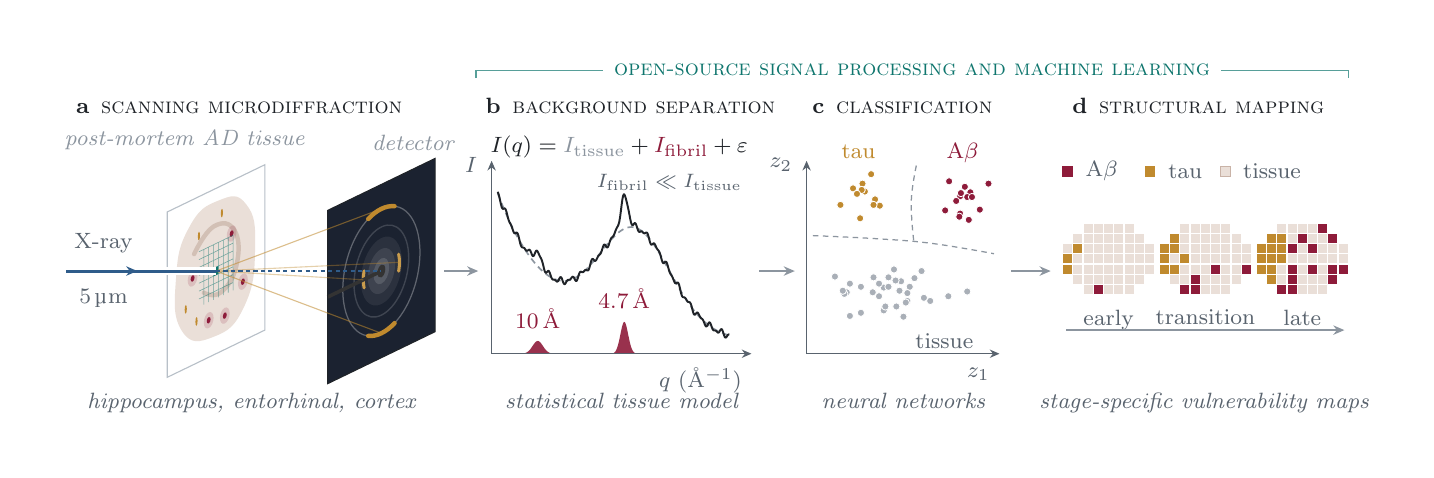
\begin{tikzpicture}[
    font=\footnotesize, text=ink,
    show background rectangle,
    background rectangle/.style={fill=white},
    inner frame sep=10pt,
    title/.style={anchor=base west, font=\footnotesize},
    sub/.style={anchor=base, text=mute, font=\footnotesize\itshape},
    tag/.style={anchor=north, text=faint, font=\footnotesize\itshape},
    axis/.style={draw=mute, line width=0.45pt, -{Stealth[length=3.5pt, width=3pt]}},
    flow/.style={draw=faint, line width=0.6pt, -{Stealth[length=4pt, width=3.4pt]}},
    declare function={
      B(\q) = 1.55*exp(-2.2*(\q-0.25)) + 0.95*exp(-pow((\q-1.42)/0.42,2)) + 0.12;
      F(\q) = 0.30*exp(-pow((\q-1.337)/0.045,2)) + 0.12*exp(-pow((\q-0.628)/0.06,2));
      N(\q) = 0.022*sin(4100*\q) + 0.015*sin(7100*\q + 40);
      X(\q) = (\q-0.25)*1.55;
    }]

  % ---------------------------------------------------------------- titles
  \node[title] at (-0.35,4.05) {\textbf{a}\enspace\textsc{scanning microdiffraction}};
  \node[title] at (4.85,4.05)  {\textbf{b}\enspace\textsc{background separation}};
  \node[title] at (9.00,4.05)  {\textbf{c}\enspace\textsc{classification}};
  \node[title] at (12.30,4.05) {\textbf{d}\enspace\textsc{structural mapping}};
  \draw[ml!70, line width=0.5pt] (4.85,4.50) -- ++(0,0.10) -| (15.93,4.50);
  \node[ml, font=\footnotesize\scshape, fill=white, inner xsep=4pt] at (10.39,4.60)
    {open-source signal processing and machine learning};

  % ---------------------------------------------------- a: experiment
  \begin{scope}[yshift=-0.20cm]
  \begin{scope}[cm={0.62,0.30,0,1,(3.65,2.25)}]               % detector
    \fill[det] (-1.1,-1.1) rectangle (1.1,1.1);
    \foreach \r/\o in {0.42/0.07, 0.28/0.09, 0.16/0.13}
      \fill[white, opacity=\o] (0,0) circle (\r);
    \draw[white, opacity=0.16, line width=0.5pt] (0,0) circle (0.56);
    \draw[white, opacity=0.30, line width=0.45pt] (0,0) circle (0.79);
    \foreach \a in {70,250}
      \draw[tau, line width=1.6pt, line cap=round]
        (\a:0.79) arc[start angle=\a, end angle=\a+40, radius=0.79];
    \foreach \a in {-17,163}
      \draw[tau!85, line width=1.1pt, line cap=round]
        (\a:0.37) arc[start angle=\a, end angle=\a+34, radius=0.37];
    \draw[black!80, line width=1.3pt] (0,0) -- (-1.1,0);
    \fill[black!80] (0,0) circle (0.08);
    \draw[ink, line width=0.4pt] (-1.1,-1.1) rectangle (1.1,1.1);
  \end{scope}

  \begin{scope}[cm={0.62,0.30,0,1,(1.55,2.25)}]               % tissue section
    \fill[white] (-1,-1.05) rectangle (1,1.05);
    \fill[tissue] plot[smooth cycle, tension=0.85] coordinates
      {(-0.70,-0.55) (-0.82,0.15) (-0.55,0.72) (0.05,0.88)
       (0.62,0.66) (0.80,0.05) (0.58,-0.62) (-0.05,-0.82)};
    \draw[tissueline, line width=1.6pt, line cap=round, opacity=0.7]
      plot[smooth, tension=0.8] coordinates
      {(-0.45,0.35) (-0.05,0.58) (0.38,0.40) (0.42,-0.05) (0.10,-0.30) (-0.25,-0.20)};
    \foreach \u/\v in {0.32/0.38, -0.48/0.05, 0.55/-0.30, -0.15/-0.58, 0.18/-0.62} {
      \fill[abeta, opacity=0.16] (\u,\v) circle (0.10);
      \fill[abeta] (\u,\v) circle (0.040);
    }
    \foreach \u/\v in {-0.35/0.55, 0.12/0.70, -0.62/-0.30, -0.40/-0.52}
      \fill[tau] (\u,\v) ellipse[x radius=0.022, y radius=0.055];
    \begin{scope}[shift={(-0.05,-0.05)}]
      \draw[ml, line width=0.2pt, opacity=0.55] (-0.3,-0.3) grid[step=0.1] (0.4,0.4);
    \end{scope}
    \fill[ml] (-0.05,-0.05) rectangle (0.05,0.05);
    \draw[rule!80!mute, line width=0.4pt] (-1,-1.05) rectangle (1,1.05);
  \end{scope}

  \foreach \p in {(3.65,3.04), (3.65,1.46)}                     % scattered rays
    \draw[tau, opacity=0.55, line width=0.4pt] (1.55,2.25) -- \p;
  \foreach \s in {1,-1}
    \draw[tau, opacity=0.40, line width=0.4pt]
      (1.55,2.25) -- ({3.65+\s*0.62*0.37},{2.25+\s*0.30*0.37});
  \draw[xray, line width=0.5pt, dash pattern=on 1.5pt off 1.2pt] (1.55,2.25) -- (3.65,2.25);
  \draw[white, line width=2.6pt] (-0.35,2.25) -- (1.55,2.25);   % incident beam
  \draw[xray, line width=1.1pt] (-0.35,2.25) -- (1.55,2.25);
  \draw[xray, line width=1.1pt, -{Stealth[length=4pt, width=3.4pt]}] (-0.35,2.25) -- (0.55,2.25);

  \node[anchor=south, text=mute] at (0.12,2.36) {X-ray};
  \node[anchor=north, text=mute] at (0.12,2.14) {5\,\textmu m};
  \node[tag, anchor=south] at (1.15,3.66) {post-mortem AD tissue};
  \node[tag, anchor=south] at (4.05,3.66) {detector};

  \end{scope}

  % ---------------------------------------- b: background separation
  \begin{scope}[shift={(5.05,1.00)}]
    \fill[abeta, opacity=0.9] plot[domain=0.3:2.2, samples=300] ({X(\x)},{1.35*F(\x)})
      -- ({X(2.2)},0) -- ({X(0.3)},0) -- cycle;
    \draw[faint, line width=0.6pt, dash pattern=on 2.2pt off 1.6pt]
      plot[domain=0.3:2.2, samples=150, smooth] ({X(\x)},{1.35*B(\x)});
    \draw[ink, line width=0.7pt, line join=round]
      plot[domain=0.3:2.2, samples=300] ({X(\x)},{1.35*(B(\x)+F(\x)+N(\x))});
    \draw[axis] (0,0) -- (3.30,0);
    \draw[axis] (0,0) -- (0,2.45);
    \node[anchor=north east, text=mute] at (3.30,-0.06) {$q$ (\AA$^{-1}$)};
    \node[anchor=east, text=mute] at (-0.06,2.40) {$I$};
    \node[anchor=south, text=abeta] at ({X(1.337)},0.45) {4.7\,\AA};
    \node[anchor=south, text=abeta] at ({X(0.628)},0.20) {10\,\AA};
    \node[anchor=north east, text=mute, font=\scriptsize] at (3.30,2.40) {$I_{\text{fibril}} \ll I_{\text{tissue}}$};
    \node at (1.62,2.62)
      {$I(q) = \textcolor{faint}{I_{\text{tissue}}} + \textcolor{abeta}{I_{\text{fibril}}} + \varepsilon$};
  \end{scope}

  % ---------------------------------------------- c: classification
  \begin{scope}[shift={(9.05,1.00)}]
    \draw[faint, line width=0.45pt, dash pattern=on 2pt off 1.6pt]
      plot[smooth, tension=0.7] coordinates {(0.08,1.50) (0.90,1.46) (1.60,1.40) (2.38,1.27)};
    \draw[faint, line width=0.45pt, dash pattern=on 2pt off 1.6pt]
      plot[smooth, tension=0.7] coordinates {(1.36,1.44) (1.33,1.95) (1.40,2.42)};
    \foreach \x/\y in {0.55/0.89, 1.28/0.67, 0.51/0.78, 1.11/1.07, 0.55/0.48, 1.18/0.92,
        1.46/1.05, 0.92/0.73, 1.8/0.73, 0.69/0.52, 0.98/0.84, 0.84/0.78, 1.04/0.97,
        1.31/0.85, 0.36/0.98, 0.48/0.76, 0.46/0.8, 0.69/0.85, 2.04/0.79, 1.23/0.47,
        0.85/0.97, 0.92/0.89, 0.98/0.55, 1.14/0.6, 1.57/0.67, 1.18/0.8, 1.26/0.65,
        1.28/0.77, 1.37/0.96, 1.0/0.6, 1.2/0.92, 1.49/0.71, 1.13/0.93, 1.04/0.85}
      \fill[faint!75, draw=white, line width=0.3pt] (\x,\y) circle (0.046);
    \foreach \x/\y in {1.95/1.78, 1.76/1.82, 2.01/2.12, 2.08/2.05, 2.04/1.99, 1.95/2.0,
        2.2/1.83, 1.81/2.19, 1.96/2.04, 2.06/1.7, 2.31/2.16, 1.94/1.74, 1.9/1.94, 2.1/1.99}
      \fill[abeta, draw=white, line width=0.3pt] (\x,\y) circle (0.046);
    \foreach \x/\y in {0.71/2.16, 0.59/2.1, 0.87/1.96, 0.43/1.89, 0.74/2.06, 0.93/1.88,
        0.7/2.08, 0.68/1.72, 0.82/2.28, 0.85/1.89, 0.64/2.03}
      \fill[tau, draw=white, line width=0.3pt] (\x,\y) circle (0.046);
    \draw[axis] (0,0) -- (2.45,0);
    \draw[axis] (0,0) -- (0,2.45);
    \node[anchor=north east, text=mute] at (2.45,-0.06) {$z_1$};
    \node[anchor=east, text=mute] at (-0.06,2.40) {$z_2$};
    \node[anchor=south, text=abeta] at (1.98,2.30) {A$\beta$};
    \node[anchor=south, text=tau] at (0.66,2.36) {tau};
    \node[anchor=north, text=mute] at (1.75,0.38) {tissue};
  \end{scope}

  % ------------------------------------------- d: structural mapping
  \begin{scope}[shift={(12.30,1.00)}]
    \foreach \c/\t/\x in {abeta/A$\beta$/0.00, tau/tau/1.05, tissue/tissue/2.00} {
      \fill[\c] (\x,2.25) rectangle ++(0.13,0.13);
      \node[anchor=west, text=mute] at (\x+0.17,2.315) {\t};
    }
    \draw[tissueline, line width=0.3pt] (2.00,2.25) rectangle ++(0.13,0.13);
    \begin{scope}[shift={(0,0.62)}]
      \foreach \i/\j/\c in {0/3/tau, 0/4/tau, 0/5/tissue, 1/2/tissue, 1/3/tissue, 1/4/tissue,
          1/5/tau, 1/6/tissue, 2/1/tissue, 2/2/tissue, 2/3/tissue, 2/4/tissue, 2/5/tissue,
          2/6/tissue, 2/7/tissue, 3/1/abeta, 3/2/tissue, 3/3/tissue, 3/4/tissue, 3/5/tissue,
          3/6/tissue, 3/7/tissue, 4/1/tissue, 4/2/tissue, 4/3/tissue, 4/4/tissue, 4/5/tissue,
          4/6/tissue, 4/7/tissue, 5/1/tissue, 5/2/tissue, 5/3/tissue, 5/4/tissue, 5/5/tissue,
          5/6/tissue, 5/7/tissue, 6/1/tissue, 6/2/tissue, 6/3/tissue, 6/4/tissue, 6/5/tissue,
          6/6/tissue, 6/7/tissue, 7/2/tissue, 7/3/tissue, 7/4/tissue, 7/5/tissue, 7/6/tissue,
          8/3/tissue, 8/4/tissue, 8/5/tissue}
        \fill[\c] (0.13*\i+0.008,0.13*\j+0.008) rectangle ++(0.114,0.114);
    \end{scope}
    \begin{scope}[shift={(1.23,0.62)}]
      \foreach \i/\j/\c in {0/3/tau, 0/4/tau, 0/5/tau, 1/2/tissue, 1/3/tau, 1/4/tissue,
          1/5/tau, 1/6/tau, 2/1/abeta, 2/2/tissue, 2/3/tissue, 2/4/tau, 2/5/tissue,
          2/6/tissue, 2/7/tissue, 3/1/abeta, 3/2/abeta, 3/3/tissue, 3/4/tissue, 3/5/tissue,
          3/6/tissue, 3/7/tissue, 4/1/tissue, 4/2/tissue, 4/3/tissue, 4/4/tissue, 4/5/tissue,
          4/6/tissue, 4/7/tissue, 5/1/tissue, 5/2/tissue, 5/3/abeta, 5/4/tissue, 5/5/tissue,
          5/6/tissue, 5/7/tissue, 6/1/tissue, 6/2/tissue, 6/3/tissue, 6/4/tissue, 6/5/tissue,
          6/6/tissue, 6/7/tissue, 7/2/tissue, 7/3/tissue, 7/4/tissue, 7/5/tissue, 7/6/tissue,
          8/3/abeta, 8/4/tissue, 8/5/tissue}
        \fill[\c] (0.13*\i+0.008,0.13*\j+0.008) rectangle ++(0.114,0.114);
    \end{scope}
    \begin{scope}[shift={(2.46,0.62)}]
      \foreach \i/\j/\c in {0/3/tau, 0/4/tau, 0/5/tau, 1/2/tau, 1/3/tau, 1/4/tau,
          1/5/tau, 1/6/tau, 2/1/abeta, 2/2/tissue, 2/3/tissue, 2/4/tau, 2/5/tau,
          2/6/tau, 2/7/tissue, 3/1/abeta, 3/2/abeta, 3/3/abeta, 3/4/tissue, 3/5/abeta,
          3/6/tissue, 3/7/tissue, 4/1/tissue, 4/2/tissue, 4/3/tissue, 4/4/tissue, 4/5/tissue,
          4/6/abeta, 4/7/tissue, 5/1/tissue, 5/2/tissue, 5/3/abeta, 5/4/tissue, 5/5/abeta,
          5/6/tissue, 5/7/tissue, 6/1/tissue, 6/2/tissue, 6/3/tissue, 6/4/tissue, 6/5/tissue,
          6/6/tissue, 6/7/abeta, 7/2/abeta, 7/3/abeta, 7/4/tissue, 7/5/tissue, 7/6/abeta,
          8/3/abeta, 8/4/tissue, 8/5/tissue}
        \fill[\c] (0.13*\i+0.008,0.13*\j+0.008) rectangle ++(0.114,0.114);
    \end{scope}
    \foreach \t/\x in {early/0.585, transition/1.815, late/3.045}
      \node[anchor=north, text=mute] at (\x,0.68) {\t};
    \draw[flow] (0.05,0.30) -- (3.58,0.30);
  \end{scope}

  % ------------------------------------------------------- panel notes
  \node[sub] at (2.00,0.30)  {hippocampus, entorhinal, cortex};
  \node[sub] at (6.70,0.30)  {statistical tissue model};
  \node[sub] at (10.28,0.30) {neural networks};
  \node[sub] at (14.10,0.30) {stage-specific vulnerability maps};

  \draw[flow] (4.45,2.05) -- (4.88,2.05);
  \draw[flow] (8.45,2.05) -- (8.90,2.05);
  \draw[flow] (11.65,2.05) -- (12.15,2.05);

\end{tikzpicture}
\end{document}
"
%          dvisvgm --no-fonts --exact-bbox --optimize research_alzheimers.dvi
\documentclass[tikz,border=0pt]{standalone}
\usepackage[T1]{fontenc}
\usepackage{lmodern}
\usepackage{amsmath}
\usetikzlibrary{arrows.meta,backgrounds}

\definecolor{ink}{HTML}{1F2328}
\definecolor{mute}{HTML}{59636E}
\definecolor{faint}{HTML}{8C959F}
\definecolor{rule}{HTML}{D0D7DE}
\definecolor{abeta}{HTML}{8E1B3A}
\definecolor{tau}{HTML}{C08A2E}
\definecolor{tissue}{HTML}{EADFD8}
\definecolor{tissueline}{HTML}{C9B3A7}
\definecolor{xray}{HTML}{2F5C8A}
\definecolor{ml}{HTML}{0F766E}
\definecolor{det}{HTML}{1B2230}

\begin{document}
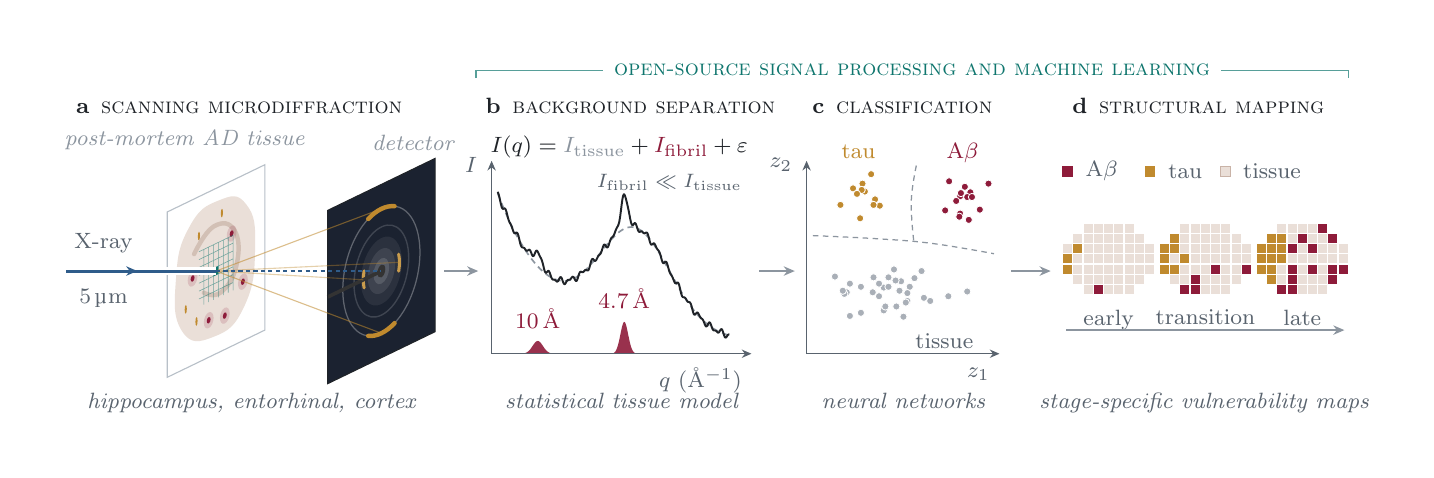
\begin{tikzpicture}[
    font=\footnotesize, text=ink,
    show background rectangle,
    background rectangle/.style={fill=white},
    inner frame sep=10pt,
    title/.style={anchor=base west, font=\footnotesize},
    sub/.style={anchor=base, text=mute, font=\footnotesize\itshape},
    tag/.style={anchor=north, text=faint, font=\footnotesize\itshape},
    axis/.style={draw=mute, line width=0.45pt, -{Stealth[length=3.5pt, width=3pt]}},
    flow/.style={draw=faint, line width=0.6pt, -{Stealth[length=4pt, width=3.4pt]}},
    declare function={
      B(\q) = 1.55*exp(-2.2*(\q-0.25)) + 0.95*exp(-pow((\q-1.42)/0.42,2)) + 0.12;
      F(\q) = 0.30*exp(-pow((\q-1.337)/0.045,2)) + 0.12*exp(-pow((\q-0.628)/0.06,2));
      N(\q) = 0.022*sin(4100*\q) + 0.015*sin(7100*\q + 40);
      X(\q) = (\q-0.25)*1.55;
    }]

  % ---------------------------------------------------------------- titles
  \node[title] at (-0.35,4.05) {\textbf{a}\enspace\textsc{scanning microdiffraction}};
  \node[title] at (4.85,4.05)  {\textbf{b}\enspace\textsc{background separation}};
  \node[title] at (9.00,4.05)  {\textbf{c}\enspace\textsc{classification}};
  \node[title] at (12.30,4.05) {\textbf{d}\enspace\textsc{structural mapping}};
  \draw[ml!70, line width=0.5pt] (4.85,4.50) -- ++(0,0.10) -| (15.93,4.50);
  \node[ml, font=\footnotesize\scshape, fill=white, inner xsep=4pt] at (10.39,4.60)
    {open-source signal processing and machine learning};

  % ---------------------------------------------------- a: experiment
  \begin{scope}[yshift=-0.20cm]
  \begin{scope}[cm={0.62,0.30,0,1,(3.65,2.25)}]               % detector
    \fill[det] (-1.1,-1.1) rectangle (1.1,1.1);
    \foreach \r/\o in {0.42/0.07, 0.28/0.09, 0.16/0.13}
      \fill[white, opacity=\o] (0,0) circle (\r);
    \draw[white, opacity=0.16, line width=0.5pt] (0,0) circle (0.56);
    \draw[white, opacity=0.30, line width=0.45pt] (0,0) circle (0.79);
    \foreach \a in {70,250}
      \draw[tau, line width=1.6pt, line cap=round]
        (\a:0.79) arc[start angle=\a, end angle=\a+40, radius=0.79];
    \foreach \a in {-17,163}
      \draw[tau!85, line width=1.1pt, line cap=round]
        (\a:0.37) arc[start angle=\a, end angle=\a+34, radius=0.37];
    \draw[black!80, line width=1.3pt] (0,0) -- (-1.1,0);
    \fill[black!80] (0,0) circle (0.08);
    \draw[ink, line width=0.4pt] (-1.1,-1.1) rectangle (1.1,1.1);
  \end{scope}

  \begin{scope}[cm={0.62,0.30,0,1,(1.55,2.25)}]               % tissue section
    \fill[white] (-1,-1.05) rectangle (1,1.05);
    \fill[tissue] plot[smooth cycle, tension=0.85] coordinates
      {(-0.70,-0.55) (-0.82,0.15) (-0.55,0.72) (0.05,0.88)
       (0.62,0.66) (0.80,0.05) (0.58,-0.62) (-0.05,-0.82)};
    \draw[tissueline, line width=1.6pt, line cap=round, opacity=0.7]
      plot[smooth, tension=0.8] coordinates
      {(-0.45,0.35) (-0.05,0.58) (0.38,0.40) (0.42,-0.05) (0.10,-0.30) (-0.25,-0.20)};
    \foreach \u/\v in {0.32/0.38, -0.48/0.05, 0.55/-0.30, -0.15/-0.58, 0.18/-0.62} {
      \fill[abeta, opacity=0.16] (\u,\v) circle (0.10);
      \fill[abeta] (\u,\v) circle (0.040);
    }
    \foreach \u/\v in {-0.35/0.55, 0.12/0.70, -0.62/-0.30, -0.40/-0.52}
      \fill[tau] (\u,\v) ellipse[x radius=0.022, y radius=0.055];
    \begin{scope}[shift={(-0.05,-0.05)}]
      \draw[ml, line width=0.2pt, opacity=0.55] (-0.3,-0.3) grid[step=0.1] (0.4,0.4);
    \end{scope}
    \fill[ml] (-0.05,-0.05) rectangle (0.05,0.05);
    \draw[rule!80!mute, line width=0.4pt] (-1,-1.05) rectangle (1,1.05);
  \end{scope}

  \foreach \p in {(3.65,3.04), (3.65,1.46)}                     % scattered rays
    \draw[tau, opacity=0.55, line width=0.4pt] (1.55,2.25) -- \p;
  \foreach \s in {1,-1}
    \draw[tau, opacity=0.40, line width=0.4pt]
      (1.55,2.25) -- ({3.65+\s*0.62*0.37},{2.25+\s*0.30*0.37});
  \draw[xray, line width=0.5pt, dash pattern=on 1.5pt off 1.2pt] (1.55,2.25) -- (3.65,2.25);
  \draw[white, line width=2.6pt] (-0.35,2.25) -- (1.55,2.25);   % incident beam
  \draw[xray, line width=1.1pt] (-0.35,2.25) -- (1.55,2.25);
  \draw[xray, line width=1.1pt, -{Stealth[length=4pt, width=3.4pt]}] (-0.35,2.25) -- (0.55,2.25);

  \node[anchor=south, text=mute] at (0.12,2.36) {X-ray};
  \node[anchor=north, text=mute] at (0.12,2.14) {5\,\textmu m};
  \node[tag, anchor=south] at (1.15,3.66) {post-mortem AD tissue};
  \node[tag, anchor=south] at (4.05,3.66) {detector};

  \end{scope}

  % ---------------------------------------- b: background separation
  \begin{scope}[shift={(5.05,1.00)}]
    \fill[abeta, opacity=0.9] plot[domain=0.3:2.2, samples=300] ({X(\x)},{1.35*F(\x)})
      -- ({X(2.2)},0) -- ({X(0.3)},0) -- cycle;
    \draw[faint, line width=0.6pt, dash pattern=on 2.2pt off 1.6pt]
      plot[domain=0.3:2.2, samples=150, smooth] ({X(\x)},{1.35*B(\x)});
    \draw[ink, line width=0.7pt, line join=round]
      plot[domain=0.3:2.2, samples=300] ({X(\x)},{1.35*(B(\x)+F(\x)+N(\x))});
    \draw[axis] (0,0) -- (3.30,0);
    \draw[axis] (0,0) -- (0,2.45);
    \node[anchor=north east, text=mute] at (3.30,-0.06) {$q$ (\AA$^{-1}$)};
    \node[anchor=east, text=mute] at (-0.06,2.40) {$I$};
    \node[anchor=south, text=abeta] at ({X(1.337)},0.45) {4.7\,\AA};
    \node[anchor=south, text=abeta] at ({X(0.628)},0.20) {10\,\AA};
    \node[anchor=north east, text=mute, font=\scriptsize] at (3.30,2.40) {$I_{\text{fibril}} \ll I_{\text{tissue}}$};
    \node at (1.62,2.62)
      {$I(q) = \textcolor{faint}{I_{\text{tissue}}} + \textcolor{abeta}{I_{\text{fibril}}} + \varepsilon$};
  \end{scope}

  % ---------------------------------------------- c: classification
  \begin{scope}[shift={(9.05,1.00)}]
    \draw[faint, line width=0.45pt, dash pattern=on 2pt off 1.6pt]
      plot[smooth, tension=0.7] coordinates {(0.08,1.50) (0.90,1.46) (1.60,1.40) (2.38,1.27)};
    \draw[faint, line width=0.45pt, dash pattern=on 2pt off 1.6pt]
      plot[smooth, tension=0.7] coordinates {(1.36,1.44) (1.33,1.95) (1.40,2.42)};
    \foreach \x/\y in {0.55/0.89, 1.28/0.67, 0.51/0.78, 1.11/1.07, 0.55/0.48, 1.18/0.92,
        1.46/1.05, 0.92/0.73, 1.8/0.73, 0.69/0.52, 0.98/0.84, 0.84/0.78, 1.04/0.97,
        1.31/0.85, 0.36/0.98, 0.48/0.76, 0.46/0.8, 0.69/0.85, 2.04/0.79, 1.23/0.47,
        0.85/0.97, 0.92/0.89, 0.98/0.55, 1.14/0.6, 1.57/0.67, 1.18/0.8, 1.26/0.65,
        1.28/0.77, 1.37/0.96, 1.0/0.6, 1.2/0.92, 1.49/0.71, 1.13/0.93, 1.04/0.85}
      \fill[faint!75, draw=white, line width=0.3pt] (\x,\y) circle (0.046);
    \foreach \x/\y in {1.95/1.78, 1.76/1.82, 2.01/2.12, 2.08/2.05, 2.04/1.99, 1.95/2.0,
        2.2/1.83, 1.81/2.19, 1.96/2.04, 2.06/1.7, 2.31/2.16, 1.94/1.74, 1.9/1.94, 2.1/1.99}
      \fill[abeta, draw=white, line width=0.3pt] (\x,\y) circle (0.046);
    \foreach \x/\y in {0.71/2.16, 0.59/2.1, 0.87/1.96, 0.43/1.89, 0.74/2.06, 0.93/1.88,
        0.7/2.08, 0.68/1.72, 0.82/2.28, 0.85/1.89, 0.64/2.03}
      \fill[tau, draw=white, line width=0.3pt] (\x,\y) circle (0.046);
    \draw[axis] (0,0) -- (2.45,0);
    \draw[axis] (0,0) -- (0,2.45);
    \node[anchor=north east, text=mute] at (2.45,-0.06) {$z_1$};
    \node[anchor=east, text=mute] at (-0.06,2.40) {$z_2$};
    \node[anchor=south, text=abeta] at (1.98,2.30) {A$\beta$};
    \node[anchor=south, text=tau] at (0.66,2.36) {tau};
    \node[anchor=north, text=mute] at (1.75,0.38) {tissue};
  \end{scope}

  % ------------------------------------------- d: structural mapping
  \begin{scope}[shift={(12.30,1.00)}]
    \foreach \c/\t/\x in {abeta/A$\beta$/0.00, tau/tau/1.05, tissue/tissue/2.00} {
      \fill[\c] (\x,2.25) rectangle ++(0.13,0.13);
      \node[anchor=west, text=mute] at (\x+0.17,2.315) {\t};
    }
    \draw[tissueline, line width=0.3pt] (2.00,2.25) rectangle ++(0.13,0.13);
    \begin{scope}[shift={(0,0.62)}]
      \foreach \i/\j/\c in {0/3/tau, 0/4/tau, 0/5/tissue, 1/2/tissue, 1/3/tissue, 1/4/tissue,
          1/5/tau, 1/6/tissue, 2/1/tissue, 2/2/tissue, 2/3/tissue, 2/4/tissue, 2/5/tissue,
          2/6/tissue, 2/7/tissue, 3/1/abeta, 3/2/tissue, 3/3/tissue, 3/4/tissue, 3/5/tissue,
          3/6/tissue, 3/7/tissue, 4/1/tissue, 4/2/tissue, 4/3/tissue, 4/4/tissue, 4/5/tissue,
          4/6/tissue, 4/7/tissue, 5/1/tissue, 5/2/tissue, 5/3/tissue, 5/4/tissue, 5/5/tissue,
          5/6/tissue, 5/7/tissue, 6/1/tissue, 6/2/tissue, 6/3/tissue, 6/4/tissue, 6/5/tissue,
          6/6/tissue, 6/7/tissue, 7/2/tissue, 7/3/tissue, 7/4/tissue, 7/5/tissue, 7/6/tissue,
          8/3/tissue, 8/4/tissue, 8/5/tissue}
        \fill[\c] (0.13*\i+0.008,0.13*\j+0.008) rectangle ++(0.114,0.114);
    \end{scope}
    \begin{scope}[shift={(1.23,0.62)}]
      \foreach \i/\j/\c in {0/3/tau, 0/4/tau, 0/5/tau, 1/2/tissue, 1/3/tau, 1/4/tissue,
          1/5/tau, 1/6/tau, 2/1/abeta, 2/2/tissue, 2/3/tissue, 2/4/tau, 2/5/tissue,
          2/6/tissue, 2/7/tissue, 3/1/abeta, 3/2/abeta, 3/3/tissue, 3/4/tissue, 3/5/tissue,
          3/6/tissue, 3/7/tissue, 4/1/tissue, 4/2/tissue, 4/3/tissue, 4/4/tissue, 4/5/tissue,
          4/6/tissue, 4/7/tissue, 5/1/tissue, 5/2/tissue, 5/3/abeta, 5/4/tissue, 5/5/tissue,
          5/6/tissue, 5/7/tissue, 6/1/tissue, 6/2/tissue, 6/3/tissue, 6/4/tissue, 6/5/tissue,
          6/6/tissue, 6/7/tissue, 7/2/tissue, 7/3/tissue, 7/4/tissue, 7/5/tissue, 7/6/tissue,
          8/3/abeta, 8/4/tissue, 8/5/tissue}
        \fill[\c] (0.13*\i+0.008,0.13*\j+0.008) rectangle ++(0.114,0.114);
    \end{scope}
    \begin{scope}[shift={(2.46,0.62)}]
      \foreach \i/\j/\c in {0/3/tau, 0/4/tau, 0/5/tau, 1/2/tau, 1/3/tau, 1/4/tau,
          1/5/tau, 1/6/tau, 2/1/abeta, 2/2/tissue, 2/3/tissue, 2/4/tau, 2/5/tau,
          2/6/tau, 2/7/tissue, 3/1/abeta, 3/2/abeta, 3/3/abeta, 3/4/tissue, 3/5/abeta,
          3/6/tissue, 3/7/tissue, 4/1/tissue, 4/2/tissue, 4/3/tissue, 4/4/tissue, 4/5/tissue,
          4/6/abeta, 4/7/tissue, 5/1/tissue, 5/2/tissue, 5/3/abeta, 5/4/tissue, 5/5/abeta,
          5/6/tissue, 5/7/tissue, 6/1/tissue, 6/2/tissue, 6/3/tissue, 6/4/tissue, 6/5/tissue,
          6/6/tissue, 6/7/abeta, 7/2/abeta, 7/3/abeta, 7/4/tissue, 7/5/tissue, 7/6/abeta,
          8/3/abeta, 8/4/tissue, 8/5/tissue}
        \fill[\c] (0.13*\i+0.008,0.13*\j+0.008) rectangle ++(0.114,0.114);
    \end{scope}
    \foreach \t/\x in {early/0.585, transition/1.815, late/3.045}
      \node[anchor=north, text=mute] at (\x,0.68) {\t};
    \draw[flow] (0.05,0.30) -- (3.58,0.30);
  \end{scope}

  % ------------------------------------------------------- panel notes
  \node[sub] at (2.00,0.30)  {hippocampus, entorhinal, cortex};
  \node[sub] at (6.70,0.30)  {statistical tissue model};
  \node[sub] at (10.28,0.30) {neural networks};
  \node[sub] at (14.10,0.30) {stage-specific vulnerability maps};

  \draw[flow] (4.45,2.05) -- (4.88,2.05);
  \draw[flow] (8.45,2.05) -- (8.90,2.05);
  \draw[flow] (11.65,2.05) -- (12.15,2.05);

\end{tikzpicture}
\end{document}
"
%          dvisvgm --no-fonts --exact-bbox --optimize research_alzheimers.dvi
\documentclass[tikz,border=0pt]{standalone}
\usepackage[T1]{fontenc}
\usepackage{lmodern}
\usepackage{amsmath}
\usetikzlibrary{arrows.meta,backgrounds}

\definecolor{ink}{HTML}{1F2328}
\definecolor{mute}{HTML}{59636E}
\definecolor{faint}{HTML}{8C959F}
\definecolor{rule}{HTML}{D0D7DE}
\definecolor{abeta}{HTML}{8E1B3A}
\definecolor{tau}{HTML}{C08A2E}
\definecolor{tissue}{HTML}{EADFD8}
\definecolor{tissueline}{HTML}{C9B3A7}
\definecolor{xray}{HTML}{2F5C8A}
\definecolor{ml}{HTML}{0F766E}
\definecolor{det}{HTML}{1B2230}

\begin{document}
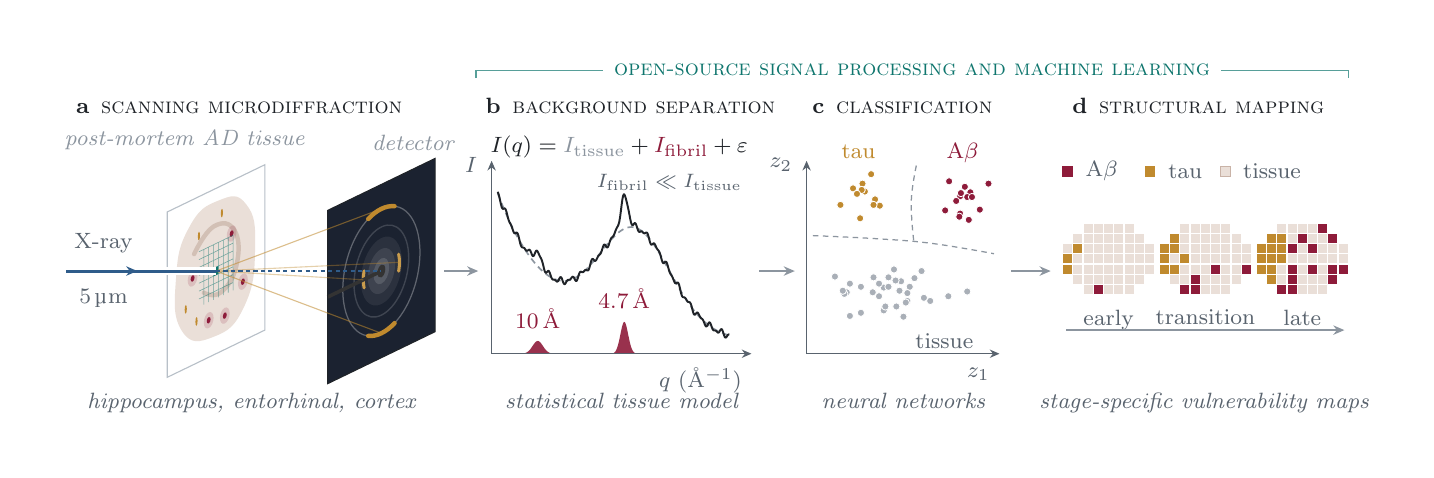
\begin{tikzpicture}[
    font=\footnotesize, text=ink,
    show background rectangle,
    background rectangle/.style={fill=white},
    inner frame sep=10pt,
    title/.style={anchor=base west, font=\footnotesize},
    sub/.style={anchor=base, text=mute, font=\footnotesize\itshape},
    tag/.style={anchor=north, text=faint, font=\footnotesize\itshape},
    axis/.style={draw=mute, line width=0.45pt, -{Stealth[length=3.5pt, width=3pt]}},
    flow/.style={draw=faint, line width=0.6pt, -{Stealth[length=4pt, width=3.4pt]}},
    declare function={
      B(\q) = 1.55*exp(-2.2*(\q-0.25)) + 0.95*exp(-pow((\q-1.42)/0.42,2)) + 0.12;
      F(\q) = 0.30*exp(-pow((\q-1.337)/0.045,2)) + 0.12*exp(-pow((\q-0.628)/0.06,2));
      N(\q) = 0.022*sin(4100*\q) + 0.015*sin(7100*\q + 40);
      X(\q) = (\q-0.25)*1.55;
    }]

  % ---------------------------------------------------------------- titles
  \node[title] at (-0.35,4.05) {\textbf{a}\enspace\textsc{scanning microdiffraction}};
  \node[title] at (4.85,4.05)  {\textbf{b}\enspace\textsc{background separation}};
  \node[title] at (9.00,4.05)  {\textbf{c}\enspace\textsc{classification}};
  \node[title] at (12.30,4.05) {\textbf{d}\enspace\textsc{structural mapping}};
  \draw[ml!70, line width=0.5pt] (4.85,4.50) -- ++(0,0.10) -| (15.93,4.50);
  \node[ml, font=\footnotesize\scshape, fill=white, inner xsep=4pt] at (10.39,4.60)
    {open-source signal processing and machine learning};

  % ---------------------------------------------------- a: experiment
  \begin{scope}[yshift=-0.20cm]
  \begin{scope}[cm={0.62,0.30,0,1,(3.65,2.25)}]               % detector
    \fill[det] (-1.1,-1.1) rectangle (1.1,1.1);
    \foreach \r/\o in {0.42/0.07, 0.28/0.09, 0.16/0.13}
      \fill[white, opacity=\o] (0,0) circle (\r);
    \draw[white, opacity=0.16, line width=0.5pt] (0,0) circle (0.56);
    \draw[white, opacity=0.30, line width=0.45pt] (0,0) circle (0.79);
    \foreach \a in {70,250}
      \draw[tau, line width=1.6pt, line cap=round]
        (\a:0.79) arc[start angle=\a, end angle=\a+40, radius=0.79];
    \foreach \a in {-17,163}
      \draw[tau!85, line width=1.1pt, line cap=round]
        (\a:0.37) arc[start angle=\a, end angle=\a+34, radius=0.37];
    \draw[black!80, line width=1.3pt] (0,0) -- (-1.1,0);
    \fill[black!80] (0,0) circle (0.08);
    \draw[ink, line width=0.4pt] (-1.1,-1.1) rectangle (1.1,1.1);
  \end{scope}

  \begin{scope}[cm={0.62,0.30,0,1,(1.55,2.25)}]               % tissue section
    \fill[white] (-1,-1.05) rectangle (1,1.05);
    \fill[tissue] plot[smooth cycle, tension=0.85] coordinates
      {(-0.70,-0.55) (-0.82,0.15) (-0.55,0.72) (0.05,0.88)
       (0.62,0.66) (0.80,0.05) (0.58,-0.62) (-0.05,-0.82)};
    \draw[tissueline, line width=1.6pt, line cap=round, opacity=0.7]
      plot[smooth, tension=0.8] coordinates
      {(-0.45,0.35) (-0.05,0.58) (0.38,0.40) (0.42,-0.05) (0.10,-0.30) (-0.25,-0.20)};
    \foreach \u/\v in {0.32/0.38, -0.48/0.05, 0.55/-0.30, -0.15/-0.58, 0.18/-0.62} {
      \fill[abeta, opacity=0.16] (\u,\v) circle (0.10);
      \fill[abeta] (\u,\v) circle (0.040);
    }
    \foreach \u/\v in {-0.35/0.55, 0.12/0.70, -0.62/-0.30, -0.40/-0.52}
      \fill[tau] (\u,\v) ellipse[x radius=0.022, y radius=0.055];
    \begin{scope}[shift={(-0.05,-0.05)}]
      \draw[ml, line width=0.2pt, opacity=0.55] (-0.3,-0.3) grid[step=0.1] (0.4,0.4);
    \end{scope}
    \fill[ml] (-0.05,-0.05) rectangle (0.05,0.05);
    \draw[rule!80!mute, line width=0.4pt] (-1,-1.05) rectangle (1,1.05);
  \end{scope}

  \foreach \p in {(3.65,3.04), (3.65,1.46)}                     % scattered rays
    \draw[tau, opacity=0.55, line width=0.4pt] (1.55,2.25) -- \p;
  \foreach \s in {1,-1}
    \draw[tau, opacity=0.40, line width=0.4pt]
      (1.55,2.25) -- ({3.65+\s*0.62*0.37},{2.25+\s*0.30*0.37});
  \draw[xray, line width=0.5pt, dash pattern=on 1.5pt off 1.2pt] (1.55,2.25) -- (3.65,2.25);
  \draw[white, line width=2.6pt] (-0.35,2.25) -- (1.55,2.25);   % incident beam
  \draw[xray, line width=1.1pt] (-0.35,2.25) -- (1.55,2.25);
  \draw[xray, line width=1.1pt, -{Stealth[length=4pt, width=3.4pt]}] (-0.35,2.25) -- (0.55,2.25);

  \node[anchor=south, text=mute] at (0.12,2.36) {X-ray};
  \node[anchor=north, text=mute] at (0.12,2.14) {5\,\textmu m};
  \node[tag, anchor=south] at (1.15,3.66) {post-mortem AD tissue};
  \node[tag, anchor=south] at (4.05,3.66) {detector};

  \end{scope}

  % ---------------------------------------- b: background separation
  \begin{scope}[shift={(5.05,1.00)}]
    \fill[abeta, opacity=0.9] plot[domain=0.3:2.2, samples=300] ({X(\x)},{1.35*F(\x)})
      -- ({X(2.2)},0) -- ({X(0.3)},0) -- cycle;
    \draw[faint, line width=0.6pt, dash pattern=on 2.2pt off 1.6pt]
      plot[domain=0.3:2.2, samples=150, smooth] ({X(\x)},{1.35*B(\x)});
    \draw[ink, line width=0.7pt, line join=round]
      plot[domain=0.3:2.2, samples=300] ({X(\x)},{1.35*(B(\x)+F(\x)+N(\x))});
    \draw[axis] (0,0) -- (3.30,0);
    \draw[axis] (0,0) -- (0,2.45);
    \node[anchor=north east, text=mute] at (3.30,-0.06) {$q$ (\AA$^{-1}$)};
    \node[anchor=east, text=mute] at (-0.06,2.40) {$I$};
    \node[anchor=south, text=abeta] at ({X(1.337)},0.45) {4.7\,\AA};
    \node[anchor=south, text=abeta] at ({X(0.628)},0.20) {10\,\AA};
    \node[anchor=north east, text=mute, font=\scriptsize] at (3.30,2.40) {$I_{\text{fibril}} \ll I_{\text{tissue}}$};
    \node at (1.62,2.62)
      {$I(q) = \textcolor{faint}{I_{\text{tissue}}} + \textcolor{abeta}{I_{\text{fibril}}} + \varepsilon$};
  \end{scope}

  % ---------------------------------------------- c: classification
  \begin{scope}[shift={(9.05,1.00)}]
    \draw[faint, line width=0.45pt, dash pattern=on 2pt off 1.6pt]
      plot[smooth, tension=0.7] coordinates {(0.08,1.50) (0.90,1.46) (1.60,1.40) (2.38,1.27)};
    \draw[faint, line width=0.45pt, dash pattern=on 2pt off 1.6pt]
      plot[smooth, tension=0.7] coordinates {(1.36,1.44) (1.33,1.95) (1.40,2.42)};
    \foreach \x/\y in {0.55/0.89, 1.28/0.67, 0.51/0.78, 1.11/1.07, 0.55/0.48, 1.18/0.92,
        1.46/1.05, 0.92/0.73, 1.8/0.73, 0.69/0.52, 0.98/0.84, 0.84/0.78, 1.04/0.97,
        1.31/0.85, 0.36/0.98, 0.48/0.76, 0.46/0.8, 0.69/0.85, 2.04/0.79, 1.23/0.47,
        0.85/0.97, 0.92/0.89, 0.98/0.55, 1.14/0.6, 1.57/0.67, 1.18/0.8, 1.26/0.65,
        1.28/0.77, 1.37/0.96, 1.0/0.6, 1.2/0.92, 1.49/0.71, 1.13/0.93, 1.04/0.85}
      \fill[faint!75, draw=white, line width=0.3pt] (\x,\y) circle (0.046);
    \foreach \x/\y in {1.95/1.78, 1.76/1.82, 2.01/2.12, 2.08/2.05, 2.04/1.99, 1.95/2.0,
        2.2/1.83, 1.81/2.19, 1.96/2.04, 2.06/1.7, 2.31/2.16, 1.94/1.74, 1.9/1.94, 2.1/1.99}
      \fill[abeta, draw=white, line width=0.3pt] (\x,\y) circle (0.046);
    \foreach \x/\y in {0.71/2.16, 0.59/2.1, 0.87/1.96, 0.43/1.89, 0.74/2.06, 0.93/1.88,
        0.7/2.08, 0.68/1.72, 0.82/2.28, 0.85/1.89, 0.64/2.03}
      \fill[tau, draw=white, line width=0.3pt] (\x,\y) circle (0.046);
    \draw[axis] (0,0) -- (2.45,0);
    \draw[axis] (0,0) -- (0,2.45);
    \node[anchor=north east, text=mute] at (2.45,-0.06) {$z_1$};
    \node[anchor=east, text=mute] at (-0.06,2.40) {$z_2$};
    \node[anchor=south, text=abeta] at (1.98,2.30) {A$\beta$};
    \node[anchor=south, text=tau] at (0.66,2.36) {tau};
    \node[anchor=north, text=mute] at (1.75,0.38) {tissue};
  \end{scope}

  % ------------------------------------------- d: structural mapping
  \begin{scope}[shift={(12.30,1.00)}]
    \foreach \c/\t/\x in {abeta/A$\beta$/0.00, tau/tau/1.05, tissue/tissue/2.00} {
      \fill[\c] (\x,2.25) rectangle ++(0.13,0.13);
      \node[anchor=west, text=mute] at (\x+0.17,2.315) {\t};
    }
    \draw[tissueline, line width=0.3pt] (2.00,2.25) rectangle ++(0.13,0.13);
    \begin{scope}[shift={(0,0.62)}]
      \foreach \i/\j/\c in {0/3/tau, 0/4/tau, 0/5/tissue, 1/2/tissue, 1/3/tissue, 1/4/tissue,
          1/5/tau, 1/6/tissue, 2/1/tissue, 2/2/tissue, 2/3/tissue, 2/4/tissue, 2/5/tissue,
          2/6/tissue, 2/7/tissue, 3/1/abeta, 3/2/tissue, 3/3/tissue, 3/4/tissue, 3/5/tissue,
          3/6/tissue, 3/7/tissue, 4/1/tissue, 4/2/tissue, 4/3/tissue, 4/4/tissue, 4/5/tissue,
          4/6/tissue, 4/7/tissue, 5/1/tissue, 5/2/tissue, 5/3/tissue, 5/4/tissue, 5/5/tissue,
          5/6/tissue, 5/7/tissue, 6/1/tissue, 6/2/tissue, 6/3/tissue, 6/4/tissue, 6/5/tissue,
          6/6/tissue, 6/7/tissue, 7/2/tissue, 7/3/tissue, 7/4/tissue, 7/5/tissue, 7/6/tissue,
          8/3/tissue, 8/4/tissue, 8/5/tissue}
        \fill[\c] (0.13*\i+0.008,0.13*\j+0.008) rectangle ++(0.114,0.114);
    \end{scope}
    \begin{scope}[shift={(1.23,0.62)}]
      \foreach \i/\j/\c in {0/3/tau, 0/4/tau, 0/5/tau, 1/2/tissue, 1/3/tau, 1/4/tissue,
          1/5/tau, 1/6/tau, 2/1/abeta, 2/2/tissue, 2/3/tissue, 2/4/tau, 2/5/tissue,
          2/6/tissue, 2/7/tissue, 3/1/abeta, 3/2/abeta, 3/3/tissue, 3/4/tissue, 3/5/tissue,
          3/6/tissue, 3/7/tissue, 4/1/tissue, 4/2/tissue, 4/3/tissue, 4/4/tissue, 4/5/tissue,
          4/6/tissue, 4/7/tissue, 5/1/tissue, 5/2/tissue, 5/3/abeta, 5/4/tissue, 5/5/tissue,
          5/6/tissue, 5/7/tissue, 6/1/tissue, 6/2/tissue, 6/3/tissue, 6/4/tissue, 6/5/tissue,
          6/6/tissue, 6/7/tissue, 7/2/tissue, 7/3/tissue, 7/4/tissue, 7/5/tissue, 7/6/tissue,
          8/3/abeta, 8/4/tissue, 8/5/tissue}
        \fill[\c] (0.13*\i+0.008,0.13*\j+0.008) rectangle ++(0.114,0.114);
    \end{scope}
    \begin{scope}[shift={(2.46,0.62)}]
      \foreach \i/\j/\c in {0/3/tau, 0/4/tau, 0/5/tau, 1/2/tau, 1/3/tau, 1/4/tau,
          1/5/tau, 1/6/tau, 2/1/abeta, 2/2/tissue, 2/3/tissue, 2/4/tau, 2/5/tau,
          2/6/tau, 2/7/tissue, 3/1/abeta, 3/2/abeta, 3/3/abeta, 3/4/tissue, 3/5/abeta,
          3/6/tissue, 3/7/tissue, 4/1/tissue, 4/2/tissue, 4/3/tissue, 4/4/tissue, 4/5/tissue,
          4/6/abeta, 4/7/tissue, 5/1/tissue, 5/2/tissue, 5/3/abeta, 5/4/tissue, 5/5/abeta,
          5/6/tissue, 5/7/tissue, 6/1/tissue, 6/2/tissue, 6/3/tissue, 6/4/tissue, 6/5/tissue,
          6/6/tissue, 6/7/abeta, 7/2/abeta, 7/3/abeta, 7/4/tissue, 7/5/tissue, 7/6/abeta,
          8/3/abeta, 8/4/tissue, 8/5/tissue}
        \fill[\c] (0.13*\i+0.008,0.13*\j+0.008) rectangle ++(0.114,0.114);
    \end{scope}
    \foreach \t/\x in {early/0.585, transition/1.815, late/3.045}
      \node[anchor=north, text=mute] at (\x,0.68) {\t};
    \draw[flow] (0.05,0.30) -- (3.58,0.30);
  \end{scope}

  % ------------------------------------------------------- panel notes
  \node[sub] at (2.00,0.30)  {hippocampus, entorhinal, cortex};
  \node[sub] at (6.70,0.30)  {statistical tissue model};
  \node[sub] at (10.28,0.30) {neural networks};
  \node[sub] at (14.10,0.30) {stage-specific vulnerability maps};

  \draw[flow] (4.45,2.05) -- (4.88,2.05);
  \draw[flow] (8.45,2.05) -- (8.90,2.05);
  \draw[flow] (11.65,2.05) -- (12.15,2.05);

\end{tikzpicture}
\end{document}
"
%          dvisvgm --no-fonts --exact-bbox --optimize research_alzheimers.dvi
\documentclass[tikz,border=0pt]{standalone}
\usepackage[T1]{fontenc}
\usepackage{lmodern}
\usepackage{amsmath}
\usetikzlibrary{arrows.meta,backgrounds}

\definecolor{ink}{HTML}{1F2328}
\definecolor{mute}{HTML}{59636E}
\definecolor{faint}{HTML}{8C959F}
\definecolor{rule}{HTML}{D0D7DE}
\definecolor{abeta}{HTML}{8E1B3A}
\definecolor{tau}{HTML}{C08A2E}
\definecolor{tissue}{HTML}{EADFD8}
\definecolor{tissueline}{HTML}{C9B3A7}
\definecolor{xray}{HTML}{2F5C8A}
\definecolor{ml}{HTML}{0F766E}
\definecolor{det}{HTML}{1B2230}

\begin{document}
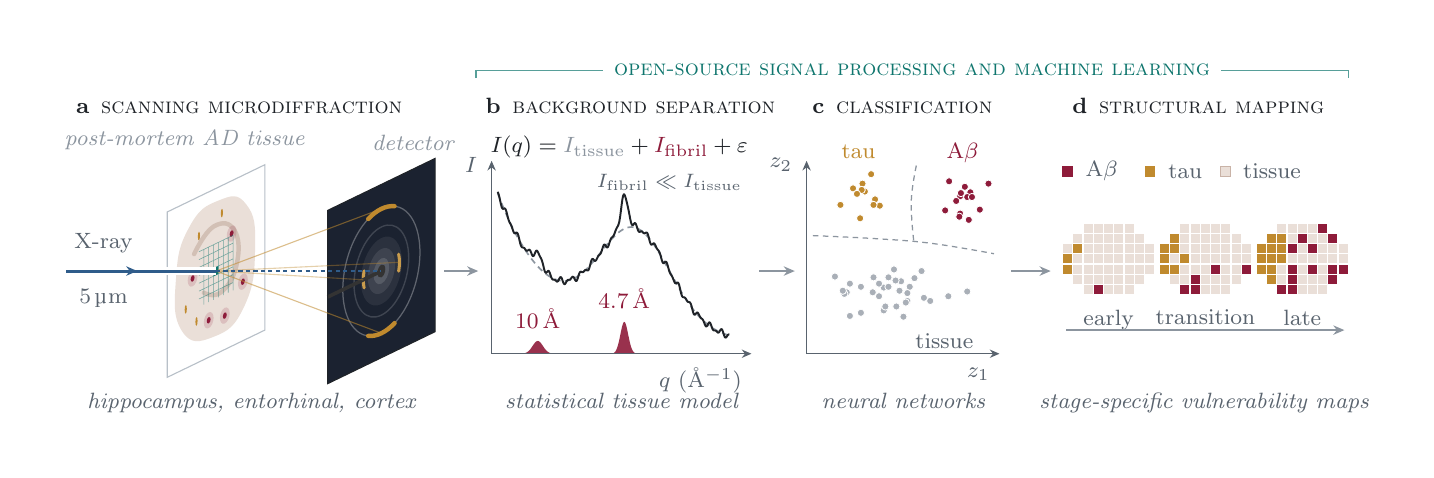
\begin{tikzpicture}[
    font=\footnotesize, text=ink,
    show background rectangle,
    background rectangle/.style={fill=white},
    inner frame sep=10pt,
    title/.style={anchor=base west, font=\footnotesize},
    sub/.style={anchor=base, text=mute, font=\footnotesize\itshape},
    tag/.style={anchor=north, text=faint, font=\footnotesize\itshape},
    axis/.style={draw=mute, line width=0.45pt, -{Stealth[length=3.5pt, width=3pt]}},
    flow/.style={draw=faint, line width=0.6pt, -{Stealth[length=4pt, width=3.4pt]}},
    declare function={
      B(\q) = 1.55*exp(-2.2*(\q-0.25)) + 0.95*exp(-pow((\q-1.42)/0.42,2)) + 0.12;
      F(\q) = 0.30*exp(-pow((\q-1.337)/0.045,2)) + 0.12*exp(-pow((\q-0.628)/0.06,2));
      N(\q) = 0.022*sin(4100*\q) + 0.015*sin(7100*\q + 40);
      X(\q) = (\q-0.25)*1.55;
    }]

  % ---------------------------------------------------------------- titles
  \node[title] at (-0.35,4.05) {\textbf{a}\enspace\textsc{scanning microdiffraction}};
  \node[title] at (4.85,4.05)  {\textbf{b}\enspace\textsc{background separation}};
  \node[title] at (9.00,4.05)  {\textbf{c}\enspace\textsc{classification}};
  \node[title] at (12.30,4.05) {\textbf{d}\enspace\textsc{structural mapping}};
  \draw[ml!70, line width=0.5pt] (4.85,4.50) -- ++(0,0.10) -| (15.93,4.50);
  \node[ml, font=\footnotesize\scshape, fill=white, inner xsep=4pt] at (10.39,4.60)
    {open-source signal processing and machine learning};

  % ---------------------------------------------------- a: experiment
  \begin{scope}[yshift=-0.20cm]
  \begin{scope}[cm={0.62,0.30,0,1,(3.65,2.25)}]               % detector
    \fill[det] (-1.1,-1.1) rectangle (1.1,1.1);
    \foreach \r/\o in {0.42/0.07, 0.28/0.09, 0.16/0.13}
      \fill[white, opacity=\o] (0,0) circle (\r);
    \draw[white, opacity=0.16, line width=0.5pt] (0,0) circle (0.56);
    \draw[white, opacity=0.30, line width=0.45pt] (0,0) circle (0.79);
    \foreach \a in {70,250}
      \draw[tau, line width=1.6pt, line cap=round]
        (\a:0.79) arc[start angle=\a, end angle=\a+40, radius=0.79];
    \foreach \a in {-17,163}
      \draw[tau!85, line width=1.1pt, line cap=round]
        (\a:0.37) arc[start angle=\a, end angle=\a+34, radius=0.37];
    \draw[black!80, line width=1.3pt] (0,0) -- (-1.1,0);
    \fill[black!80] (0,0) circle (0.08);
    \draw[ink, line width=0.4pt] (-1.1,-1.1) rectangle (1.1,1.1);
  \end{scope}

  \begin{scope}[cm={0.62,0.30,0,1,(1.55,2.25)}]               % tissue section
    \fill[white] (-1,-1.05) rectangle (1,1.05);
    \fill[tissue] plot[smooth cycle, tension=0.85] coordinates
      {(-0.70,-0.55) (-0.82,0.15) (-0.55,0.72) (0.05,0.88)
       (0.62,0.66) (0.80,0.05) (0.58,-0.62) (-0.05,-0.82)};
    \draw[tissueline, line width=1.6pt, line cap=round, opacity=0.7]
      plot[smooth, tension=0.8] coordinates
      {(-0.45,0.35) (-0.05,0.58) (0.38,0.40) (0.42,-0.05) (0.10,-0.30) (-0.25,-0.20)};
    \foreach \u/\v in {0.32/0.38, -0.48/0.05, 0.55/-0.30, -0.15/-0.58, 0.18/-0.62} {
      \fill[abeta, opacity=0.16] (\u,\v) circle (0.10);
      \fill[abeta] (\u,\v) circle (0.040);
    }
    \foreach \u/\v in {-0.35/0.55, 0.12/0.70, -0.62/-0.30, -0.40/-0.52}
      \fill[tau] (\u,\v) ellipse[x radius=0.022, y radius=0.055];
    \begin{scope}[shift={(-0.05,-0.05)}]
      \draw[ml, line width=0.2pt, opacity=0.55] (-0.3,-0.3) grid[step=0.1] (0.4,0.4);
    \end{scope}
    \fill[ml] (-0.05,-0.05) rectangle (0.05,0.05);
    \draw[rule!80!mute, line width=0.4pt] (-1,-1.05) rectangle (1,1.05);
  \end{scope}

  \foreach \p in {(3.65,3.04), (3.65,1.46)}                     % scattered rays
    \draw[tau, opacity=0.55, line width=0.4pt] (1.55,2.25) -- \p;
  \foreach \s in {1,-1}
    \draw[tau, opacity=0.40, line width=0.4pt]
      (1.55,2.25) -- ({3.65+\s*0.62*0.37},{2.25+\s*0.30*0.37});
  \draw[xray, line width=0.5pt, dash pattern=on 1.5pt off 1.2pt] (1.55,2.25) -- (3.65,2.25);
  \draw[white, line width=2.6pt] (-0.35,2.25) -- (1.55,2.25);   % incident beam
  \draw[xray, line width=1.1pt] (-0.35,2.25) -- (1.55,2.25);
  \draw[xray, line width=1.1pt, -{Stealth[length=4pt, width=3.4pt]}] (-0.35,2.25) -- (0.55,2.25);

  \node[anchor=south, text=mute] at (0.12,2.36) {X-ray};
  \node[anchor=north, text=mute] at (0.12,2.14) {5\,\textmu m};
  \node[tag, anchor=south] at (1.15,3.66) {post-mortem AD tissue};
  \node[tag, anchor=south] at (4.05,3.66) {detector};

  \end{scope}

  % ---------------------------------------- b: background separation
  \begin{scope}[shift={(5.05,1.00)}]
    \fill[abeta, opacity=0.9] plot[domain=0.3:2.2, samples=300] ({X(\x)},{1.35*F(\x)})
      -- ({X(2.2)},0) -- ({X(0.3)},0) -- cycle;
    \draw[faint, line width=0.6pt, dash pattern=on 2.2pt off 1.6pt]
      plot[domain=0.3:2.2, samples=150, smooth] ({X(\x)},{1.35*B(\x)});
    \draw[ink, line width=0.7pt, line join=round]
      plot[domain=0.3:2.2, samples=300] ({X(\x)},{1.35*(B(\x)+F(\x)+N(\x))});
    \draw[axis] (0,0) -- (3.30,0);
    \draw[axis] (0,0) -- (0,2.45);
    \node[anchor=north east, text=mute] at (3.30,-0.06) {$q$ (\AA$^{-1}$)};
    \node[anchor=east, text=mute] at (-0.06,2.40) {$I$};
    \node[anchor=south, text=abeta] at ({X(1.337)},0.45) {4.7\,\AA};
    \node[anchor=south, text=abeta] at ({X(0.628)},0.20) {10\,\AA};
    \node[anchor=north east, text=mute, font=\scriptsize] at (3.30,2.40) {$I_{\text{fibril}} \ll I_{\text{tissue}}$};
    \node at (1.62,2.62)
      {$I(q) = \textcolor{faint}{I_{\text{tissue}}} + \textcolor{abeta}{I_{\text{fibril}}} + \varepsilon$};
  \end{scope}

  % ---------------------------------------------- c: classification
  \begin{scope}[shift={(9.05,1.00)}]
    \draw[faint, line width=0.45pt, dash pattern=on 2pt off 1.6pt]
      plot[smooth, tension=0.7] coordinates {(0.08,1.50) (0.90,1.46) (1.60,1.40) (2.38,1.27)};
    \draw[faint, line width=0.45pt, dash pattern=on 2pt off 1.6pt]
      plot[smooth, tension=0.7] coordinates {(1.36,1.44) (1.33,1.95) (1.40,2.42)};
    \foreach \x/\y in {0.55/0.89, 1.28/0.67, 0.51/0.78, 1.11/1.07, 0.55/0.48, 1.18/0.92,
        1.46/1.05, 0.92/0.73, 1.8/0.73, 0.69/0.52, 0.98/0.84, 0.84/0.78, 1.04/0.97,
        1.31/0.85, 0.36/0.98, 0.48/0.76, 0.46/0.8, 0.69/0.85, 2.04/0.79, 1.23/0.47,
        0.85/0.97, 0.92/0.89, 0.98/0.55, 1.14/0.6, 1.57/0.67, 1.18/0.8, 1.26/0.65,
        1.28/0.77, 1.37/0.96, 1.0/0.6, 1.2/0.92, 1.49/0.71, 1.13/0.93, 1.04/0.85}
      \fill[faint!75, draw=white, line width=0.3pt] (\x,\y) circle (0.046);
    \foreach \x/\y in {1.95/1.78, 1.76/1.82, 2.01/2.12, 2.08/2.05, 2.04/1.99, 1.95/2.0,
        2.2/1.83, 1.81/2.19, 1.96/2.04, 2.06/1.7, 2.31/2.16, 1.94/1.74, 1.9/1.94, 2.1/1.99}
      \fill[abeta, draw=white, line width=0.3pt] (\x,\y) circle (0.046);
    \foreach \x/\y in {0.71/2.16, 0.59/2.1, 0.87/1.96, 0.43/1.89, 0.74/2.06, 0.93/1.88,
        0.7/2.08, 0.68/1.72, 0.82/2.28, 0.85/1.89, 0.64/2.03}
      \fill[tau, draw=white, line width=0.3pt] (\x,\y) circle (0.046);
    \draw[axis] (0,0) -- (2.45,0);
    \draw[axis] (0,0) -- (0,2.45);
    \node[anchor=north east, text=mute] at (2.45,-0.06) {$z_1$};
    \node[anchor=east, text=mute] at (-0.06,2.40) {$z_2$};
    \node[anchor=south, text=abeta] at (1.98,2.30) {A$\beta$};
    \node[anchor=south, text=tau] at (0.66,2.36) {tau};
    \node[anchor=north, text=mute] at (1.75,0.38) {tissue};
  \end{scope}

  % ------------------------------------------- d: structural mapping
  \begin{scope}[shift={(12.30,1.00)}]
    \foreach \c/\t/\x in {abeta/A$\beta$/0.00, tau/tau/1.05, tissue/tissue/2.00} {
      \fill[\c] (\x,2.25) rectangle ++(0.13,0.13);
      \node[anchor=west, text=mute] at (\x+0.17,2.315) {\t};
    }
    \draw[tissueline, line width=0.3pt] (2.00,2.25) rectangle ++(0.13,0.13);
    \begin{scope}[shift={(0,0.62)}]
      \foreach \i/\j/\c in {0/3/tau, 0/4/tau, 0/5/tissue, 1/2/tissue, 1/3/tissue, 1/4/tissue,
          1/5/tau, 1/6/tissue, 2/1/tissue, 2/2/tissue, 2/3/tissue, 2/4/tissue, 2/5/tissue,
          2/6/tissue, 2/7/tissue, 3/1/abeta, 3/2/tissue, 3/3/tissue, 3/4/tissue, 3/5/tissue,
          3/6/tissue, 3/7/tissue, 4/1/tissue, 4/2/tissue, 4/3/tissue, 4/4/tissue, 4/5/tissue,
          4/6/tissue, 4/7/tissue, 5/1/tissue, 5/2/tissue, 5/3/tissue, 5/4/tissue, 5/5/tissue,
          5/6/tissue, 5/7/tissue, 6/1/tissue, 6/2/tissue, 6/3/tissue, 6/4/tissue, 6/5/tissue,
          6/6/tissue, 6/7/tissue, 7/2/tissue, 7/3/tissue, 7/4/tissue, 7/5/tissue, 7/6/tissue,
          8/3/tissue, 8/4/tissue, 8/5/tissue}
        \fill[\c] (0.13*\i+0.008,0.13*\j+0.008) rectangle ++(0.114,0.114);
    \end{scope}
    \begin{scope}[shift={(1.23,0.62)}]
      \foreach \i/\j/\c in {0/3/tau, 0/4/tau, 0/5/tau, 1/2/tissue, 1/3/tau, 1/4/tissue,
          1/5/tau, 1/6/tau, 2/1/abeta, 2/2/tissue, 2/3/tissue, 2/4/tau, 2/5/tissue,
          2/6/tissue, 2/7/tissue, 3/1/abeta, 3/2/abeta, 3/3/tissue, 3/4/tissue, 3/5/tissue,
          3/6/tissue, 3/7/tissue, 4/1/tissue, 4/2/tissue, 4/3/tissue, 4/4/tissue, 4/5/tissue,
          4/6/tissue, 4/7/tissue, 5/1/tissue, 5/2/tissue, 5/3/abeta, 5/4/tissue, 5/5/tissue,
          5/6/tissue, 5/7/tissue, 6/1/tissue, 6/2/tissue, 6/3/tissue, 6/4/tissue, 6/5/tissue,
          6/6/tissue, 6/7/tissue, 7/2/tissue, 7/3/tissue, 7/4/tissue, 7/5/tissue, 7/6/tissue,
          8/3/abeta, 8/4/tissue, 8/5/tissue}
        \fill[\c] (0.13*\i+0.008,0.13*\j+0.008) rectangle ++(0.114,0.114);
    \end{scope}
    \begin{scope}[shift={(2.46,0.62)}]
      \foreach \i/\j/\c in {0/3/tau, 0/4/tau, 0/5/tau, 1/2/tau, 1/3/tau, 1/4/tau,
          1/5/tau, 1/6/tau, 2/1/abeta, 2/2/tissue, 2/3/tissue, 2/4/tau, 2/5/tau,
          2/6/tau, 2/7/tissue, 3/1/abeta, 3/2/abeta, 3/3/abeta, 3/4/tissue, 3/5/abeta,
          3/6/tissue, 3/7/tissue, 4/1/tissue, 4/2/tissue, 4/3/tissue, 4/4/tissue, 4/5/tissue,
          4/6/abeta, 4/7/tissue, 5/1/tissue, 5/2/tissue, 5/3/abeta, 5/4/tissue, 5/5/abeta,
          5/6/tissue, 5/7/tissue, 6/1/tissue, 6/2/tissue, 6/3/tissue, 6/4/tissue, 6/5/tissue,
          6/6/tissue, 6/7/abeta, 7/2/abeta, 7/3/abeta, 7/4/tissue, 7/5/tissue, 7/6/abeta,
          8/3/abeta, 8/4/tissue, 8/5/tissue}
        \fill[\c] (0.13*\i+0.008,0.13*\j+0.008) rectangle ++(0.114,0.114);
    \end{scope}
    \foreach \t/\x in {early/0.585, transition/1.815, late/3.045}
      \node[anchor=north, text=mute] at (\x,0.68) {\t};
    \draw[flow] (0.05,0.30) -- (3.58,0.30);
  \end{scope}

  % ------------------------------------------------------- panel notes
  \node[sub] at (2.00,0.30)  {hippocampus, entorhinal, cortex};
  \node[sub] at (6.70,0.30)  {statistical tissue model};
  \node[sub] at (10.28,0.30) {neural networks};
  \node[sub] at (14.10,0.30) {stage-specific vulnerability maps};

  \draw[flow] (4.45,2.05) -- (4.88,2.05);
  \draw[flow] (8.45,2.05) -- (8.90,2.05);
  \draw[flow] (11.65,2.05) -- (12.15,2.05);

\end{tikzpicture}
\end{document}
